\chapter{Problem Statement}


- prototype for a complex sensor health monitoring structure.
    -employing standardized data classes
        -metadata semantics (SOIL)
        -pandas series
    -employing standardized interfaces for modular expansions



-structuring


        %%%%%%%%%%%%%%

	• Precise detection of malfunctions and perturbances
	• Reporting tool that displays relevant info and generates metrics
Plug and play philosophy

\section{Concrete Problem}

%%%%%%%%%%%%%%%%%%%%%%%%%%%%%%%%%%%%%%%%%%%%%%%%%%%%%%
existing proposal:

Sensor Health Monitoring
Sensors fail. And have unexpected outputs. Not catching these faults can sometimes come at great costs when a research campaign proves to be useless when no sensible data has been produced. And even greater costs when the data acquisitioning systems have been changed and reconfigured for the next campaign.
To solve this, an automatical fault detection/Health Monitoring of sensors shall be investigated and developed.

Motivation and problem
To create checks, the sensors have to be checked against a configuration database. As straightforward as it sounds this proves to have some challenges to it as the existing configuration formats need to first be understood and then transformed into a format in which they can be read by the python code. Of course, this step needs to be dynamic and expandable for different configurations since the aircrafts’ configuration may change frequently.
A nomenclature and procedure can be formulated upon segmenting the problem of faulty sensors into different fault catching steps.
1.	Production of data
2.	Production of data that is within an expected range of values
3.	Production of data that acts sensible in reference to other sensors
Since metadata regarding Steps one and two like the Sensor names as well as their ranges can be defined in the configuration database, the main work to solve these procedures lies in the creation of a thorough configuration management.
Systems which simulate a dynamic model as well as neural networks or other algorithms can be implemented in step 3 for finding correlations between sensors and detecting perhaps previously unknown correlations.

Approaches
Sensor Health Monitoring is a multilayered problem whose challenges not only lie in the single operational tasks themselves but also the integration into the existing infrastructure of the sensors. Since the DLRs aircraft sensor configurations are subject to change a database shall be devised that does not create an additional location for configurations to be updated. Thus, a dynamical sensor health monitoring over changing sensor configurations is proposed that at least shall be designed with the architecture in place to enable such a design
Changing configurations may be incorporated into a standardized sensor configuration management system. Research has to be conducted on how this database of sensor metadata is going to be implemented in the best way. The SOIL system shall be examined closer for this task and rated and perhaps modified according to its’ abilities.
Once a sound sensor configuration database is found, simple checks on SHM Level 1 and 2 should be conducted without great effort. For Level 3 approaches, a systemic approach will have to be found that interfaces the sensors to a physical correlation model and then back to themselves. Simple physical correlations can be a starting point for more complex algorithms like control system approaches based upon Pseudo Transfer Functions. These would be able to reference the State Space variables to the sensor outputs without knowing the systems inputs. Also possible is the use of neural networks. However, the control systems approach is chosen first as it offers more transparency on its logic and hence facilitates the debugging process.
Once satisfying solutions are reached in a simple version of the Level 3 approaches, additional sensors may be added while recursively checking that solutions remain sensible. A possible strategy would be to rebuild the approach from Aircraft Sensor Health Monitoring for omega_z derived from omega_x, omega_y and drift angle: delta_beta. Further use of this model could be expanded once it has been proven to work.


Validation
Debugging a fault detection for aircraft with around 400 sensors will certainly prove tedious. An approach using about 10 sensors might be easier to validate. Steps 1 and 2 will not need much validation after verifying the relatively simple logic. Step 3 however will create a physical model. This model can be validated by using known physical correlations to reference sensors to the simulated model and calculate the difference over an entire flight. This in turn can be investigated to validate the method. Further validation methods may be employed later on once more is known about the topic.


\section{Methodology}

The first consideration to be taken is that this is the development of a development system. Since SHM is a multifaceted problem that represents a grand undertaking with many moving parts and optimizable parameters, algorithms and systems that may be implemented, it is firstly considered necessary to develop an ecosystem and a process in which SHM algorithms may be tested, evaluated and optimized. To develop said ecosystem, the turbine model for development of Human-Machine Systems is featured \cite{adlakha-hutcheon_human_2022}. Its process can be applied to this work without much changes. Starting from Ideation stage that represents the beginning phase as well as the first Chapter of this work. Within Ideation phase the project orientation takes place. Which goals are considered viable within the given constraints of time and manpower as well as ressources such as knowledge and available tooling.
After Ideation Phase the vertical movement representing creativity and innovational ideas is centered into a level-headed assessment of the problem containing goals and boundary conditions. Using these condensed ideas and values, the Research and Technology Assessment Phase is kicked off, represented by Chapter 2 of this work in which various technologies are examined for usage within the given problem context. Based upon a wide and thorough research feasible ideas and approaches can now be arranged within an infrastructure to solve the given problem. Fitting together various approaches from the literature like puzzle-pieces and condensing the ideas into a more refined concept, concluding literature review and representing a first draft. Using this first draft, the development cycle can now be started which can also be represented by the spiral model displayed in figure \ref{fig:spiral model}. The challenge of this third stage is now to implement the draft given in the previous stage, this gets accomplished by bouncing from an exploration step in which the theoretical constructs from the previous steps are implemented into a review step in which the systems are rated upon usability. This also represents the procedure of chapter 4 in which the theory from chapter 2 is implemented and developed. After having then developed a prototype of this work we can assess the results for our test cases (sensor failures) in chapter 5.




\begin{figure}[h]
    \centering
    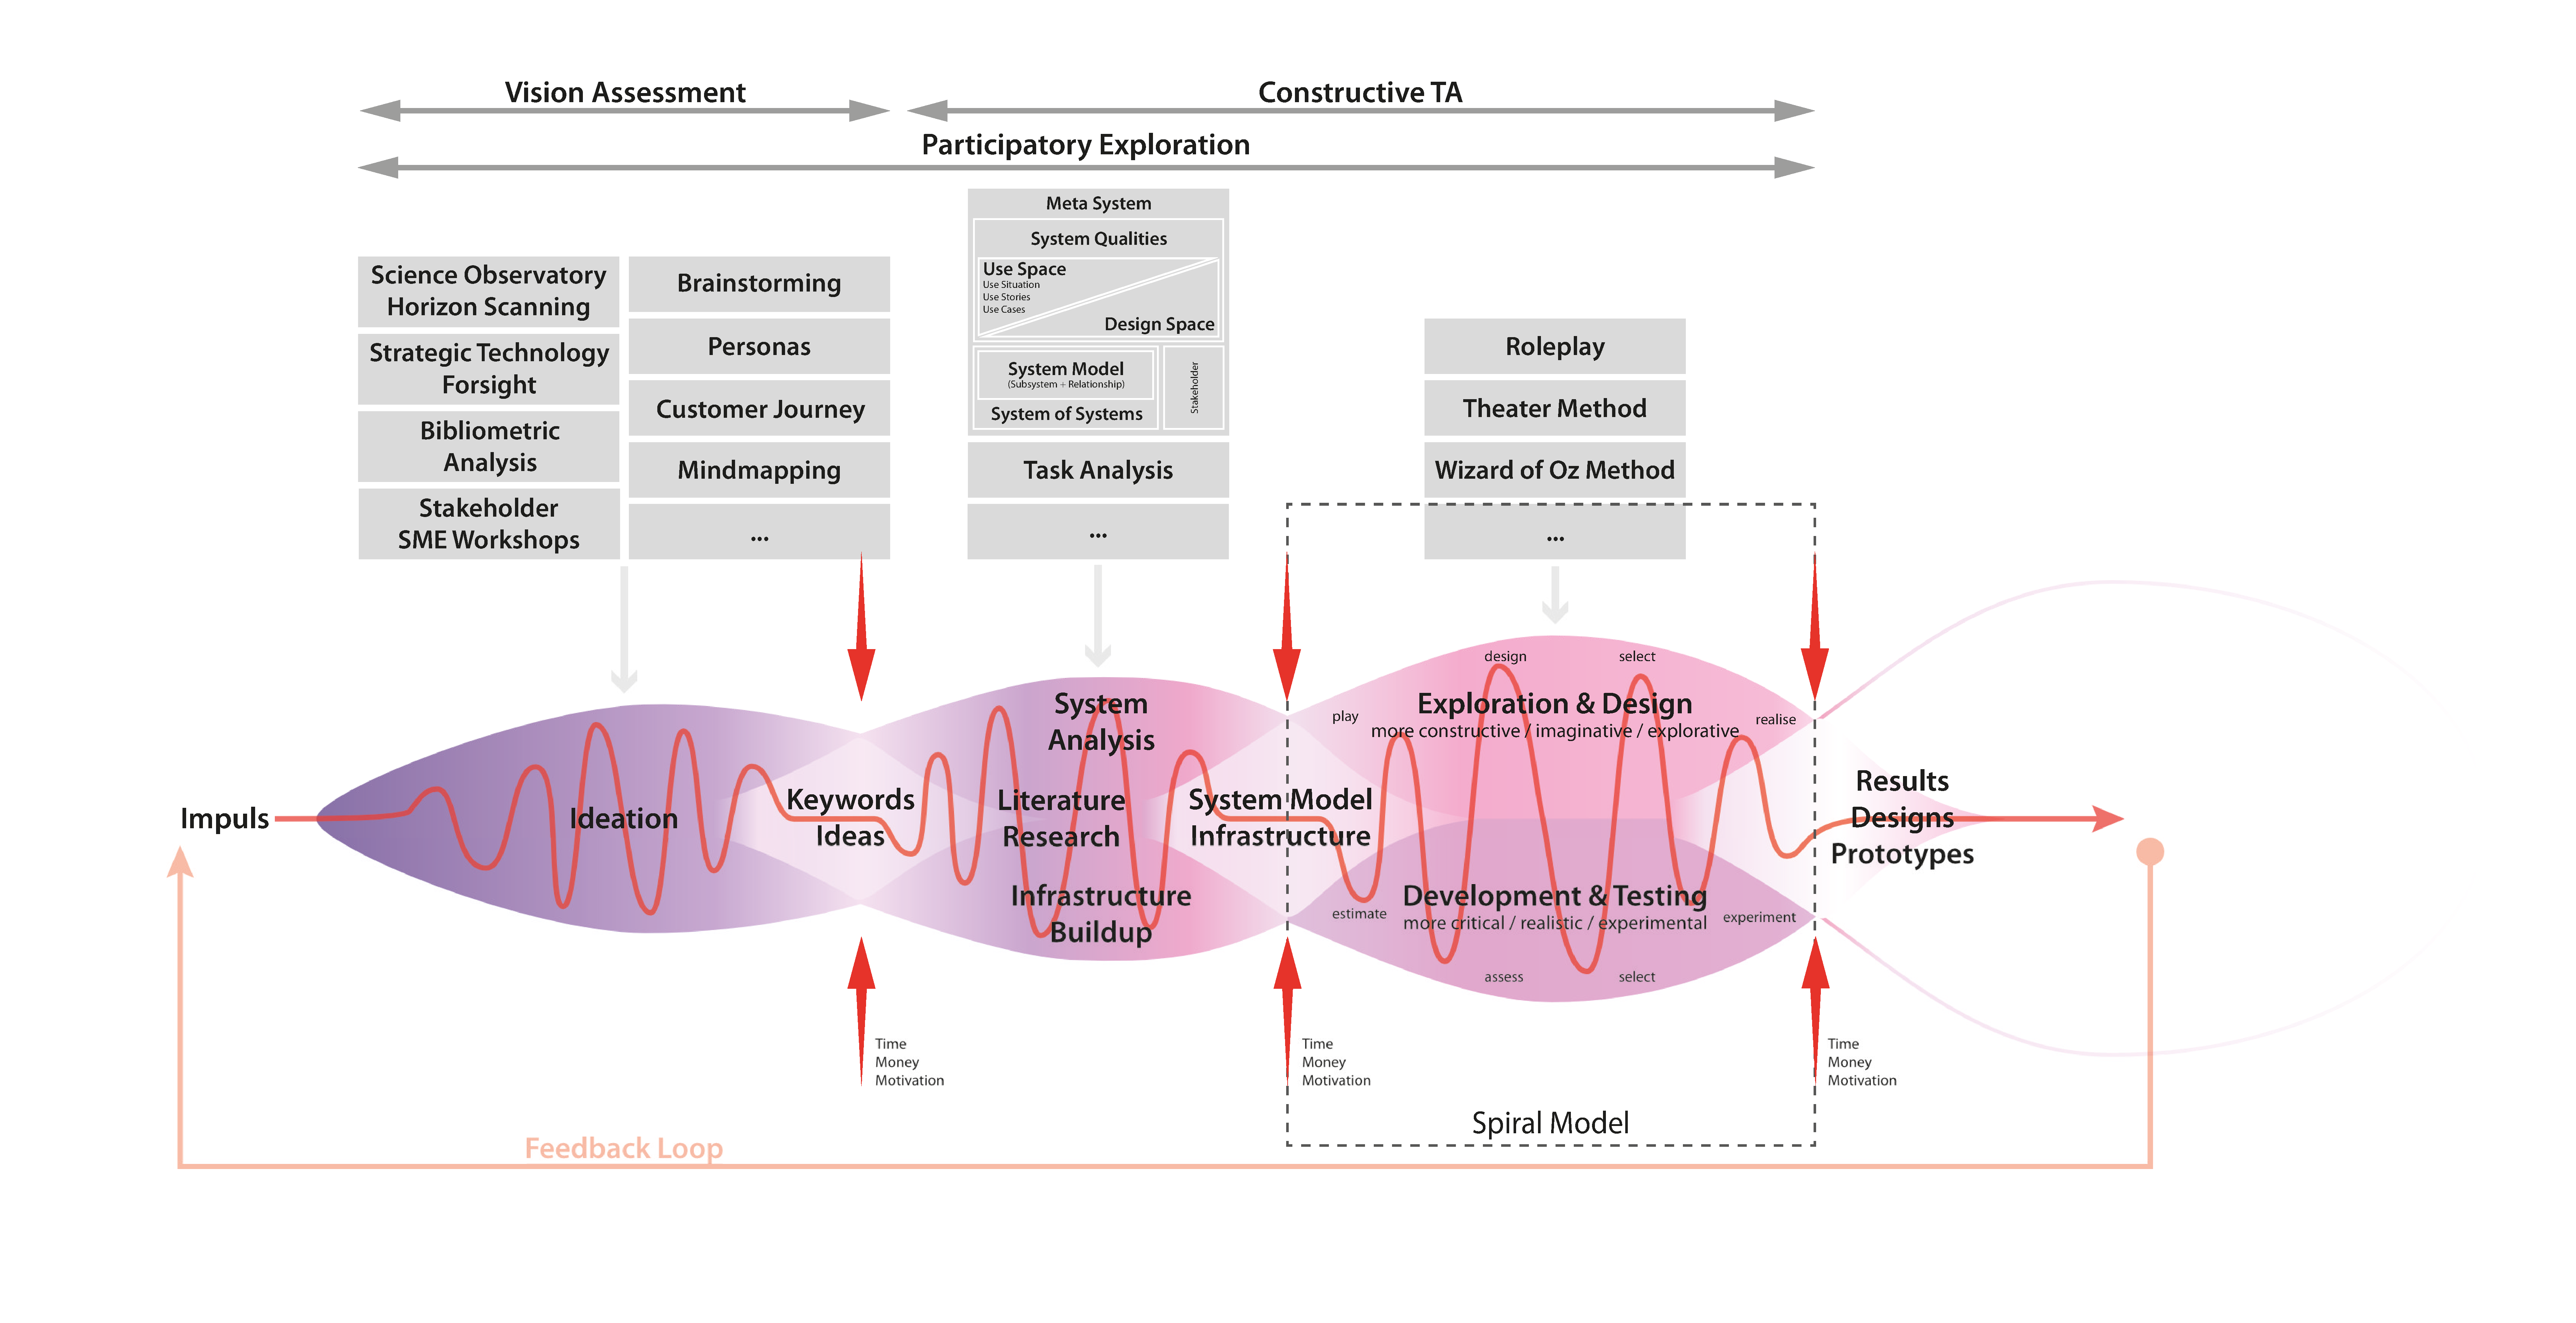
\includegraphics[width=\textwidth]{Innovationsturbine}
    \caption{The innovation and exploration turbine in the context of this work as a two times nested feedback loop. \cite{adlakha-hutcheon_human_2022}}
    \label{fig:innovation_turbine}
\end{figure}

\begin{figure}[h]
    \centering
    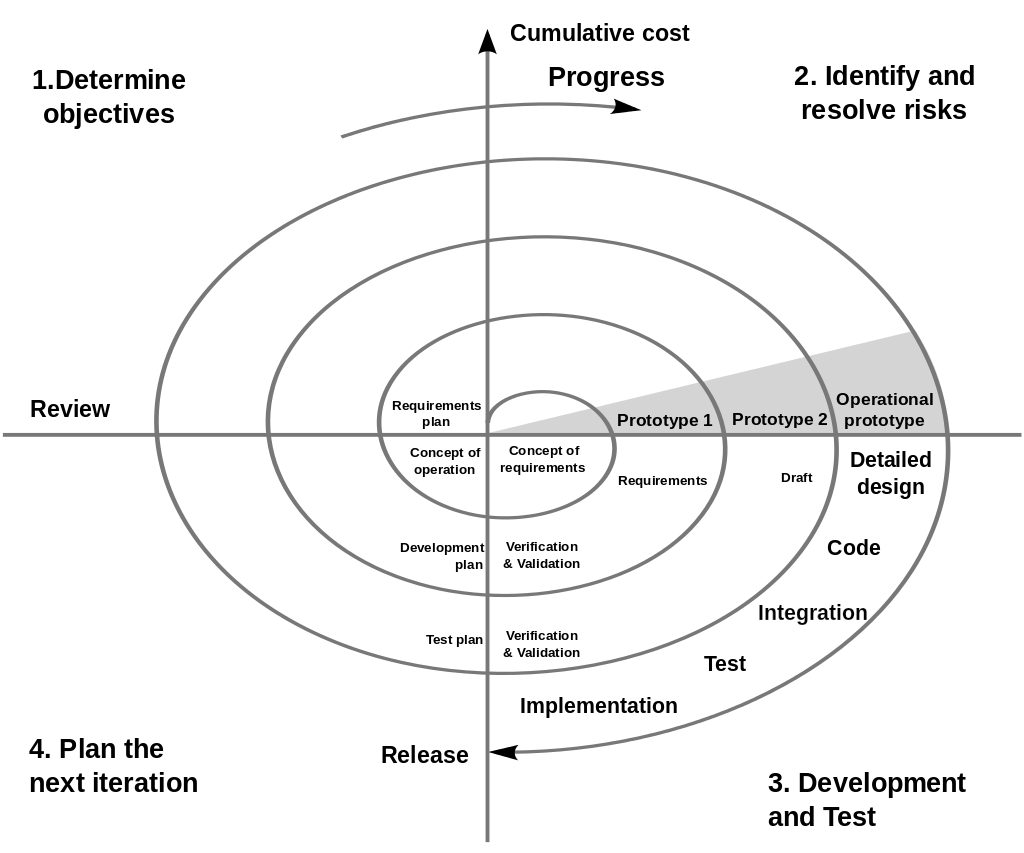
\includegraphics[width=.8\textwidth]{Spiral_model_(Boehm,_1988).svg}
    \caption{The spiral model featured within the innovation turbine \cite{boehm_spiral_1986}}
    \label{fig:spiral model}
\end{figure}


